Για την προσομοίωση γύρου, χρησιμοποιήθηκε το μοντέλο ανοιχτού κώδικα \openLap \cite{halkiopoulos_openlap_fileexchange,halkiopoulos_openlap_github} που περιλαμβάνει τον αλγόριθμο επίλυσης γύρου που περιγράφηκε στην εισαγωγή του κεφαλαίου \ref{sec:lapSim}.\\
\noindent
Οι μοναδικές επεμβάσεις που χρειάστηκαν στο \openLap ήταν οι εξής:

\paragraph{Ενσωμάτωση μοντέλου οχήματος.}
Καθώς το \openLap διαθέτει το δικό του μοντέλο οχήματος, όσοι υπολογισμοί αφορούν τη δυναμική του οχήματος, παρακάμφθηκαν, με την αντικατάστασή τους από την άμεση αναφορά στο διάγραμμα επιδόσεων του μοντέλου της παρούσας εργασίας. Συγκεκριμένα:

\begin{itemize}
    \item Για δεδομένη επιτάχυνση $a_y$, εύρεση $a_{x}^-,\ a_{x}^+$ μέσω διαγράμματος \textit{GGV}.
    \item Αφαίρεση επίδρασης οπισθέλκουσας -- το \openLap χρησιμοποιεί απλοποιημένο μοντέλο οχήματος σημειακής μάζας, το \text{GGV} του μοντέλου της εργασίας συμπεριλαμβάνει φαινόμενα της γεωμετρίας οχήματος και την επίδραση των αντιστάσεων.
\end{itemize}

\paragraph{Επίδραση θερμοκρασίας και φθοράς.}
Ένας επιλύτης \textit{QSS} δε διαθέτει την ιστορία του οχήματος κατά την επίλυση, δηλαδή, κάθε σημείο της πίστας αποτελεί ξεχωριστή κατάσταση και δεν επηρεάζεται από την προηγούμενη. Ένα πρακτικό αποτέλεσμα αυτής της παρατήρησης είναι πως κατά τον χρόνο της επίλυσης, δεν μπορεί να είναι γνωστή η εξέλιξη της θερμοκρασίας και της φθοράς.\\
\noindent
Επομένως, για να συμπεριληφθεί η επίδραση της κατάστασης του ελαστικού, χρησιμοποιείται μια (σχεδόν) επαναληπτική διαδικασία όπως περιγράφεται παρακάτω.

\begin{enumerate}
    \item Προσομοίωση ενός γύρου με σταθερές καταστάσεις ελαστικού κατά μήκος της πίστας (ίσες με τις αρχικές συνθήκες).
    \item Υπολογισμός εξέλιξης θερμοκρασίας και φθοράς, με τη μέθοδο του κεφαλαίου \ref{sec:inverseModel}.
    \label{bullet:tempReconstruction}
    \item Επανάληψη προσομοίωσης γύρου με τις καταστάσεις ελαστικού κατά μήκος της πίστας του βήματος \ref{bullet:tempReconstruction}.
\end{enumerate}

Τα βήματα \ref{bullet:tempReconstruction} και 3 θα μπορούσαν να επαναληφθούν έως να επέλθει σύγκλιση, ωστόσο, προς αποφυγή περιττών υπολογιστικών κύκλων, θεωρείται πως μια επανάληψη είναι αρκετή ώστε να αποτυπώσει την επίδραση της κατάστασης των ελαστικών στον χρόνο ενός γύρου (\cref{fig:iterT_tempPerTyre,fig:iterT_velocity}). Παρακάτω φαίνεται η σύγκριση μεταξύ της εξέλιξης της θερμοκρασίας αλλά και του προφίλ της ταχύτητας στις δύο διαδοχικές προσομοιώσεις του γύρου.

\begin{figure}[htbp!]
    \centering
    \begin{subfigure}[t]{0.48\textwidth}
        \centering
        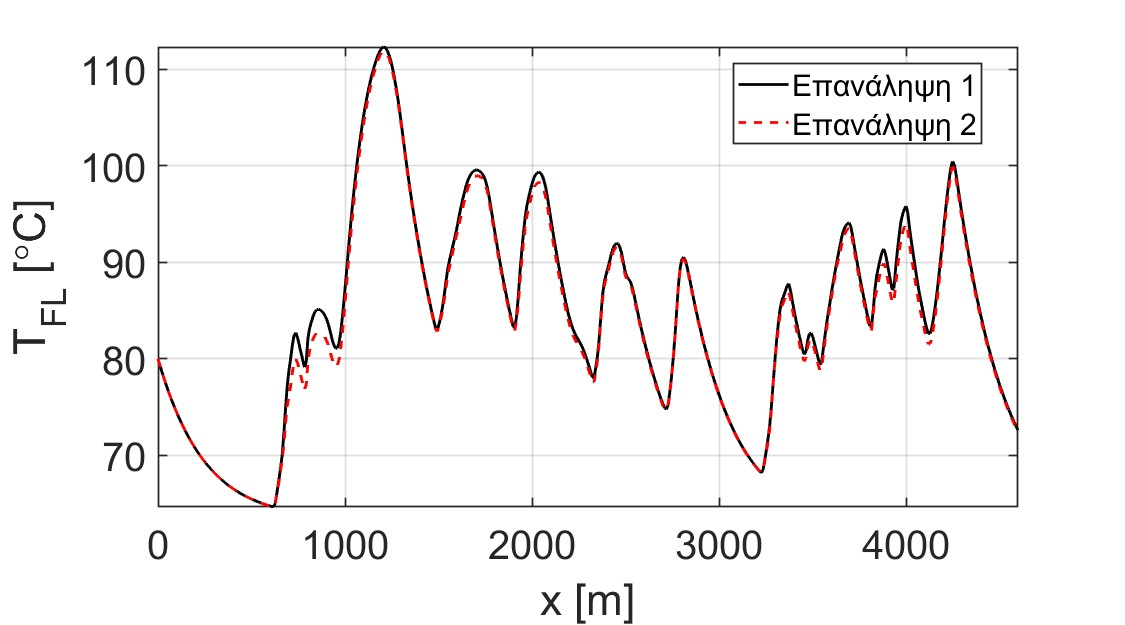
\includegraphics[width=\textwidth]{figures/iterativeT/T_convergence_FL.jpg}
    \end{subfigure}
    \hfill
    \begin{subfigure}[t]{0.48\textwidth}
        \centering
        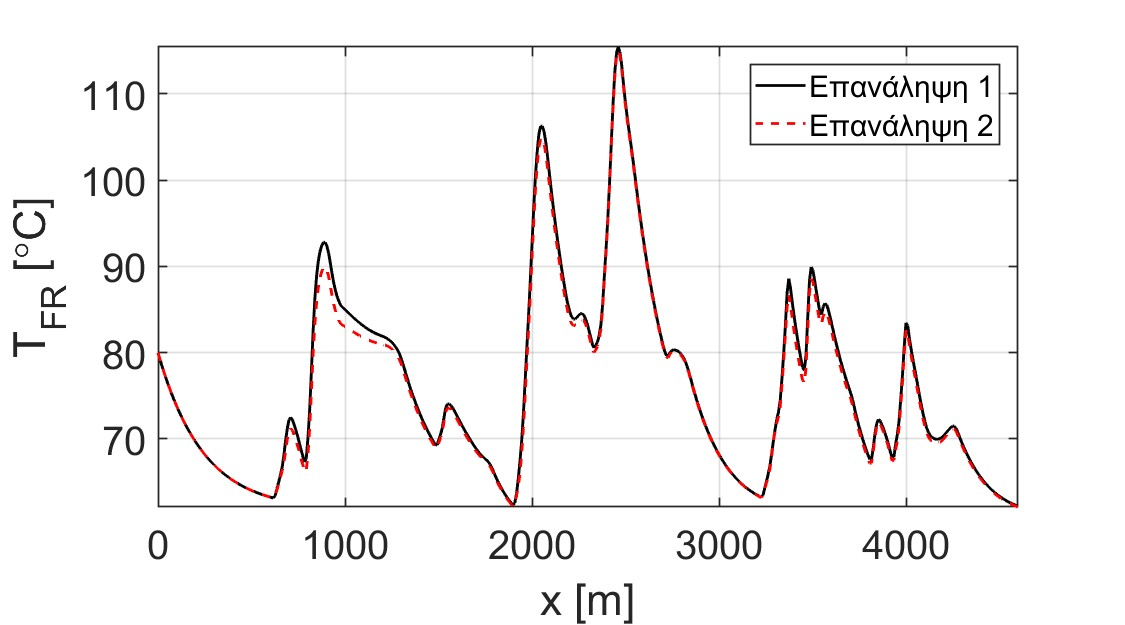
\includegraphics[width=\textwidth]{figures/iterativeT/T_convergence_FR.jpg}
    \end{subfigure}

    \vspace{0.5em}

    \begin{subfigure}[t]{0.48\textwidth}
        \centering
        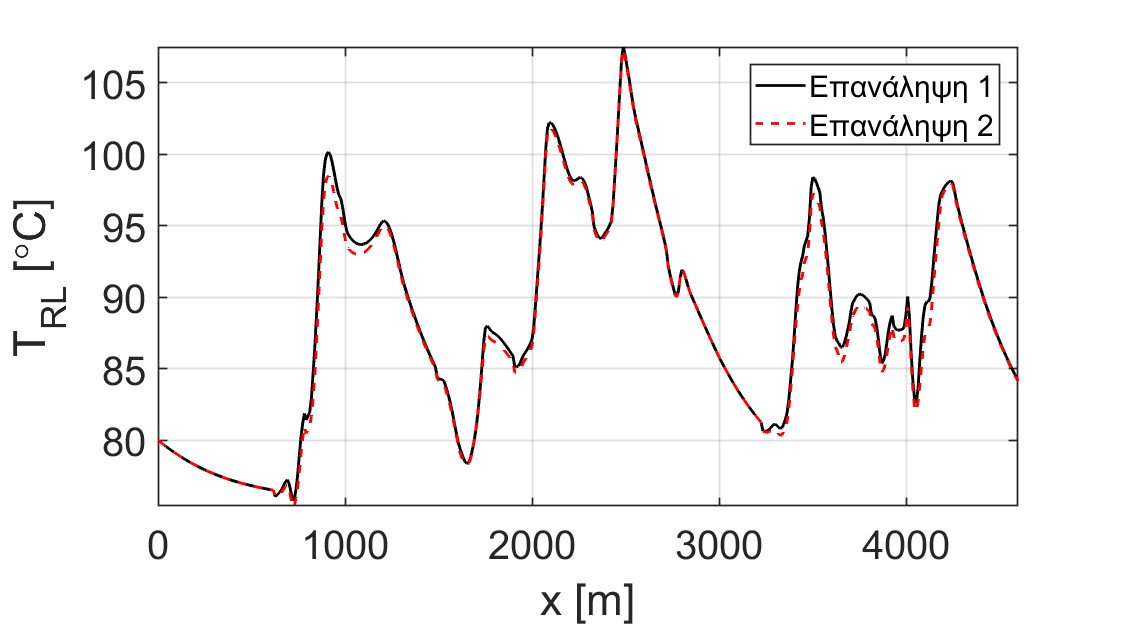
\includegraphics[width=\textwidth]{figures/iterativeT/T_convergence_RL.jpg}
    \end{subfigure}
    \hfill
    \begin{subfigure}[t]{0.48\textwidth}
        \centering
        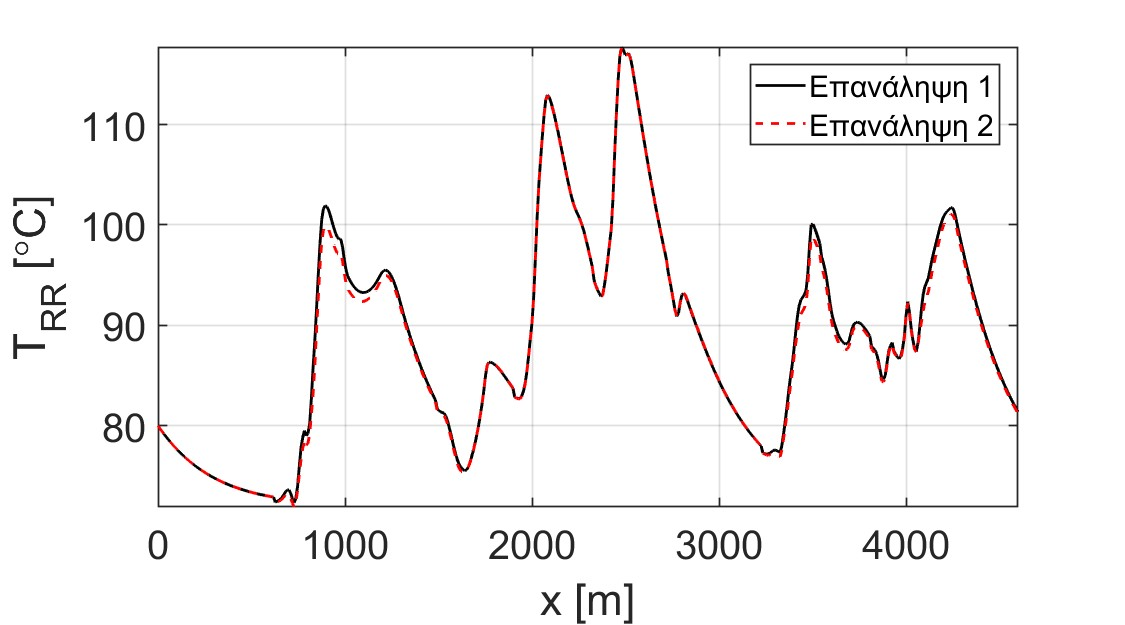
\includegraphics[width=\textwidth]{figures/iterativeT/T_convergence_RR.jpg}
    \end{subfigure}
    \caption{Σύγκριση $T_i(x)$ ανά ελαστικό ανάμεσα στην πρώτη (σταθερές συνθήκες) και στη δεύτερη επανάληψη (μεταβαλλόμενες συνθήκες).}
    \label{fig:iterT_tempPerTyre}
\end{figure}

\begin{figure}[htbp!]
    \centering
    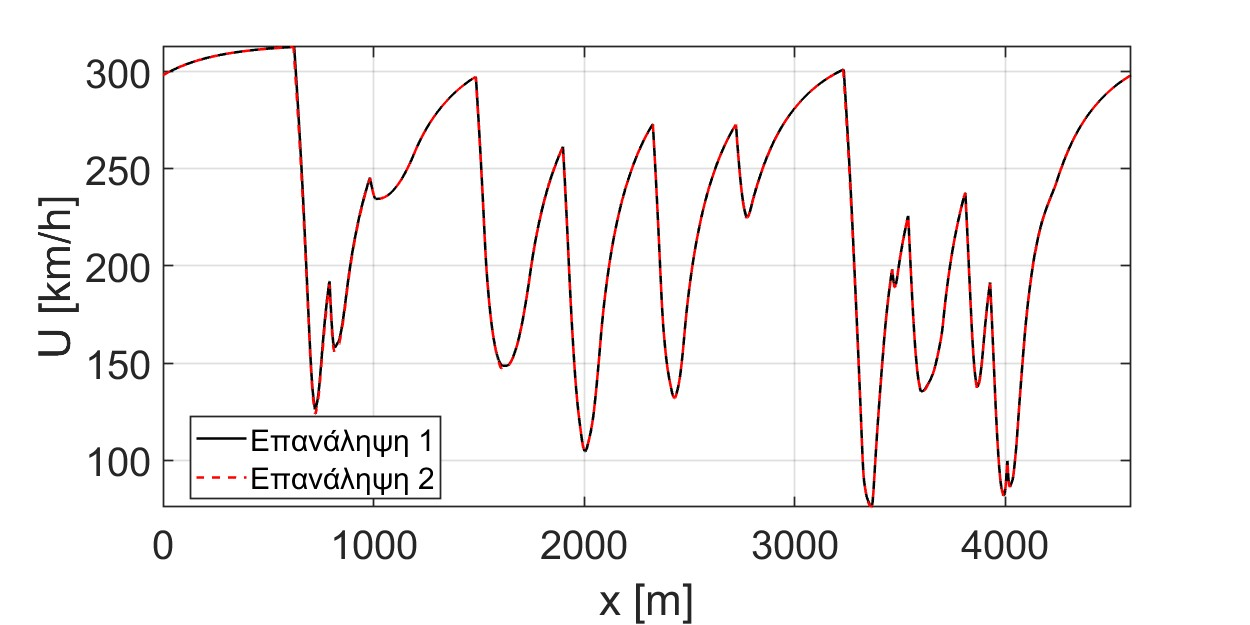
\includegraphics[width=0.85\textwidth]{figures/iterativeT/vel_iter.jpg}
    \caption{Προφίλ ταχύτητας $U(x)$ για τις δύο διαδοχικές επαναλήψεις.}
    \label{fig:iterT_velocity}
\end{figure}

\FloatBarrier


